\documentclass[a4paper, 14pt]{extarticle}

\usepackage{cmap}
\usepackage[T2A]{fontenc}
\usepackage[utf8]{inputenc}
\usepackage[english, russian]{babel}
\usepackage{amsmath}
\usepackage{subcaption}
\usepackage{graphicx}
\usepackage{multirow}
\usepackage{float}
\usepackage{placeins}
\usepackage{hyperref}

\usepackage[left=3cm, right=1.5cm, top=2cm, bottom=2cm]{geometry}
\usepackage{setspace}
\onehalfspacing 

\usepackage{indentfirst}
\setlength{\parindent}{1.25cm} 
\setlength{\emergencystretch}{3em}
\usepackage[expansion=false,protrusion=false,nopatch=footnote]{microtype}

\usepackage{tocloft}
\addto\captionsrussian{\renewcommand{\contentsname}{СОДЕРЖАНИЕ}}
\renewcommand{\cfttoctitlefont}{\hfill\normalfont}
\renewcommand{\cftaftertoctitle}{\hfill\vspace{\baselineskip}}
\renewcommand{\cftsecdotsep}{\cftdotsep}

\begin{document}

\begin{titlepage}
    \begin{center}
        Министерство науки и высшего образования Российской Федерации\\
        Федеральное государственное автономное образовательное учреждение высшего образования\\
        «Санкт-Петербургский политехнический университет Петра Великого»\\
        
        \textbf{Физико-механический институт}\\
        \textbf{Высшая школа прикладной математики и вычислительной физики}
    \end{center}

    \vfill
    
    \begin{center}
        \textbf{Отчёт по лабораторной работе \textnumero~ 4\\[0.5cm]}
        \textbf{ Эмпирическая функция распределения и ядерные оценки плотности\\}
        по дисциплине <<Математическая статистика>>
    \end{center}

    \vfill

    \hfill
    \begin{minipage}{0.45\textwidth}
        \textbf{Выполнил студент гр. 5030102/30202:}\\
        Шильдт Д.С.\\[0.5cm]
        \textbf{Преподаватель:}\\ 
        Баженов А.Н.
    \end{minipage}

    \vfill

    \begin{center}
        Санкт-Петербург\\2026
    \end{center}
\end{titlepage}

\setcounter{page}{2}

\tableofcontents
\newpage

\section{Постановка задачи}

\textbf{Цели и задачи работы:}
\begin{itemize}
    \item Освоить методы непараметрического оценивания неизвестной функции распределения и плотности вероятности по выборочным данным.
    \item Проанализировать влияние объема выборки на точность приближения теоретических кривых их эмпирическими оценками и сравнить ядерные оценки плотности с гистограммами.
\end{itemize}

\textbf{Задание:}
Сгенерировать независимые выборки объемом $n \in \{20, 60, 100\}$. Построить на них:
\begin{enumerate}
    \item Эмпирическую функцию распределения (э. ф. р.) и теоретическую функцию распределения.
    \item Ядерную оценку плотности (ядро — гауссово) и теоретическую плотность
\end{enumerate}

\section{Теоретическая часть}

Эмпирическая функция распределения $F_n^*(x)$ выступает точечной статистической оценкой теоретической функции распределения $F(x)$. Она определяет относительную частоту события $X < x$ для заданной выборки. Аналитически $F_n^*(x)$ задается как неубывающая ступенчатая функция со скачками, равными $1/n$, в каждом элементе вариационного ряда:
\begin{equation}
    F_n^*(x) = \frac{1}{n} \sum_{i=1}^n I(x_i < x),
\end{equation}
где $I(\cdot)$ — функция-индикатор, принимающая значение $1$ при выполнении условия $x_i < x$ и $0$ в противном случае. По мере неограниченного роста объема выборки $n$, согласно фундаментальным предельным теоремам, эмпирическая функция равномерно сходится к истинной $F(x)$.

Ядерная оценка плотности $\hat{f}_h(x)$ применяется для гладкого непараметрического восстановления неизвестной генеральной плотности вероятности. Вычисление базируется на суперпозиции локальных ядер:
\begin{equation}
    \hat{f}_h(x) = \frac{1}{nh} \sum_{i=1}^n K\left(\frac{x - x_i}{h}\right),
\end{equation}
где $K(u)$ — весовая ядерная функция, удовлетворяющая нормировочному условию $\int K(u) du = 1$. Стандартной практикой является использование гауссовского ядра $K(u) = \frac{1}{\sqrt{2\pi}} e^{-u^2/2}$.

Степень гладкости итоговой кривой определяется параметром ширины полосы $h$. При недостаточном $h$ график покрывается высокочастотными флуктуациями (недосглаживание), при избыточном — теряет структурные особенности распределения (пересглаживание). Оптимальный шаг интегрирования, минимизирующий среднеквадратичную ошибку, вычисляется по эмпирическому правилу Сильвермана:
\begin{equation}
    h = 1.06 \cdot \hat{\sigma} \cdot n^{-1/5},
\end{equation}
где $\hat{\sigma}$ — выборочное стандартное отклонение. 

Специфика дискретных законов исключает применение непрерывного ядерного сглаживания. Для распределения Пуассона $P(5)$ непрерывная оценка плотности лишена математического смысла, поэтому её аналогом на графиках выступает полигон относительных частот.

\section{Реализация}

\subsection{Язык программирования и среда}
    \begin{itemize}
        \item \textbf{Используемый язык:} Python 3.14.2
        \item \textbf{Используемая среда разработки:} Visual Studio Code
    \end{itemize}

\subsection{Используемые библиотеки}
    \begin{itemize}
        \item \textbf{numpy} --- использовалась для работы с массивами данных, сортировки выборок, вычисления сеток значений и агрегирования метрик.
        \item \textbf{scipy} --- использовалась для генерации выборок из теоретических распределений и вычисления функций распределения/плотности.
        \item \textbf{matplotlib} --- использовалась для построения графиков эмпирической функции распределения, ядерной оценки плотности и сохранения итоговых рисунков.
        \item \textbf{pathlib} --- использовалась для автоматического создания каталогов и записи итоговых PNG-файлов и CSV-таблицы.
    \end{itemize}

\subsection{Суть реализованных методов}

\begin{itemize}
    \item \texttt{getDistributionConfigs()} --- формирует список исследуемых распределений и задает для каждого из них генератор выборки, теоретическую функцию распределения и теоретическую плотность.
    \item \texttt{makeEcdf(sample)} --- строит эмпирическую функцию распределения по отсортированной выборке и возвращает вариационный ряд вместе с накопленными относительными частотами.
    \item \texttt{plotEcdf(ax, sample, config, sample\_size)} --- выводит на одном графике эмпирическую и теоретическую функции распределения для выбранного объема выборки.
    \item \texttt{plotDensity(ax, sample, config, sample\_size)} --- строит ядерную оценку плотности для непрерывных распределений; для Пуассона используется полигон относительных частот и теоретическая вероятность.
    \item \texttt{computeErrorMetrics(sample, config)} --- вычисляет максимальное отклонение эмпирической функции распределения от теоретической и среднеквадратичную ошибку оценки плотности.
    \item \texttt{saveDistributionFigure(config, rng)} --- формирует итоговый рисунок для одного распределения и сохраняет его в каталог \texttt{figures}.
    \item \texttt{saveCsv(rows)} и \texttt{printReport(rows)} --- отвечают за экспорт численных результатов в файл \texttt{ecdf\_kde\_metrics.csv} и вывод сводки в консоль.
\end{itemize}

\section{Результаты}

В ходе статистического моделирования для каждого распределения построены отдельные блоки графиков: сначала показаны эмпирическая и теоретическая функции распределения, ниже --- оценка плотности и теоретическая плотность (рис.~\ref{fig:norm_pair}--\ref{fig:uniform_pair}). 

Количественные метрики отклонений эмпирических кривых от теоретических представлены в таблице \ref{tab:ecdf_kde}. Значения округлены до четырех знаков после запятой.

\begin{table}[H]
    \centering
    \caption{Метрики отклонения эмпирических оценок от теоретических функций}
    \label{tab:ecdf_kde}
    \small
    \resizebox{\textwidth}{!}{%
    \begin{tabular}{|l|c|c|c|}
        \hline
        \textbf{Распределение} & $\mathbf{n}$ & $\mathbf{\max |F_n^*(x) - F(x)|}$ & $\mathbf{MSE}$ \textbf{плотности} \\ \hline
        \multirow{3}{*}{Нормальное $N(0, 1)$} 
        & 20 & 0.1300 & 0.0011 \\ \cline{2-4}
        & 60 & 0.1089 & 0.0015 \\ \cline{2-4}
        & 100 & 0.1216 & 0.0010 \\ \hline
        \multirow{3}{*}{Коши $C(0, 1)$} 
        & 20 & 0.1338 & 0.0041 \\ \cline{2-4}
        & 60 & 0.0867 & 0.0048 \\ \cline{2-4}
        & 100 & 0.0580 & 0.0028 \\ \hline
        \multirow{3}{*}{Лапласа $L(0, 1/\sqrt{2})$} 
        & 20 & 0.1142 & 0.0016 \\ \cline{2-4}
        & 60 & 0.1287 & 0.0065 \\ \cline{2-4}
        & 100 & 0.0676 & 0.0008 \\ \hline
        \multirow{3}{*}{Пуассона $P(5)$} 
        & 20 & 0.0819 & 0.0004 \\ \cline{2-4}
        & 60 & 0.0348 & 0.0001 \\ \cline{2-4}
        & 100 & 0.0478 & 0.0007 \\ \hline
        \multirow{3}{*}{Равномерное $U(-\sqrt{3}, \sqrt{3})$} 
        & 20 & 0.1698 & 0.0032 \\ \cline{2-4}
        & 60 & 0.1337 & 0.0023 \\ \cline{2-4}
        & 100 & 0.0513 & 0.0020 \\ \hline
    \end{tabular}
    }
\end{table}
\begin{figure}[!htbp]
    \centering
    \begin{subfigure}[t]{\textwidth}
        \centering
        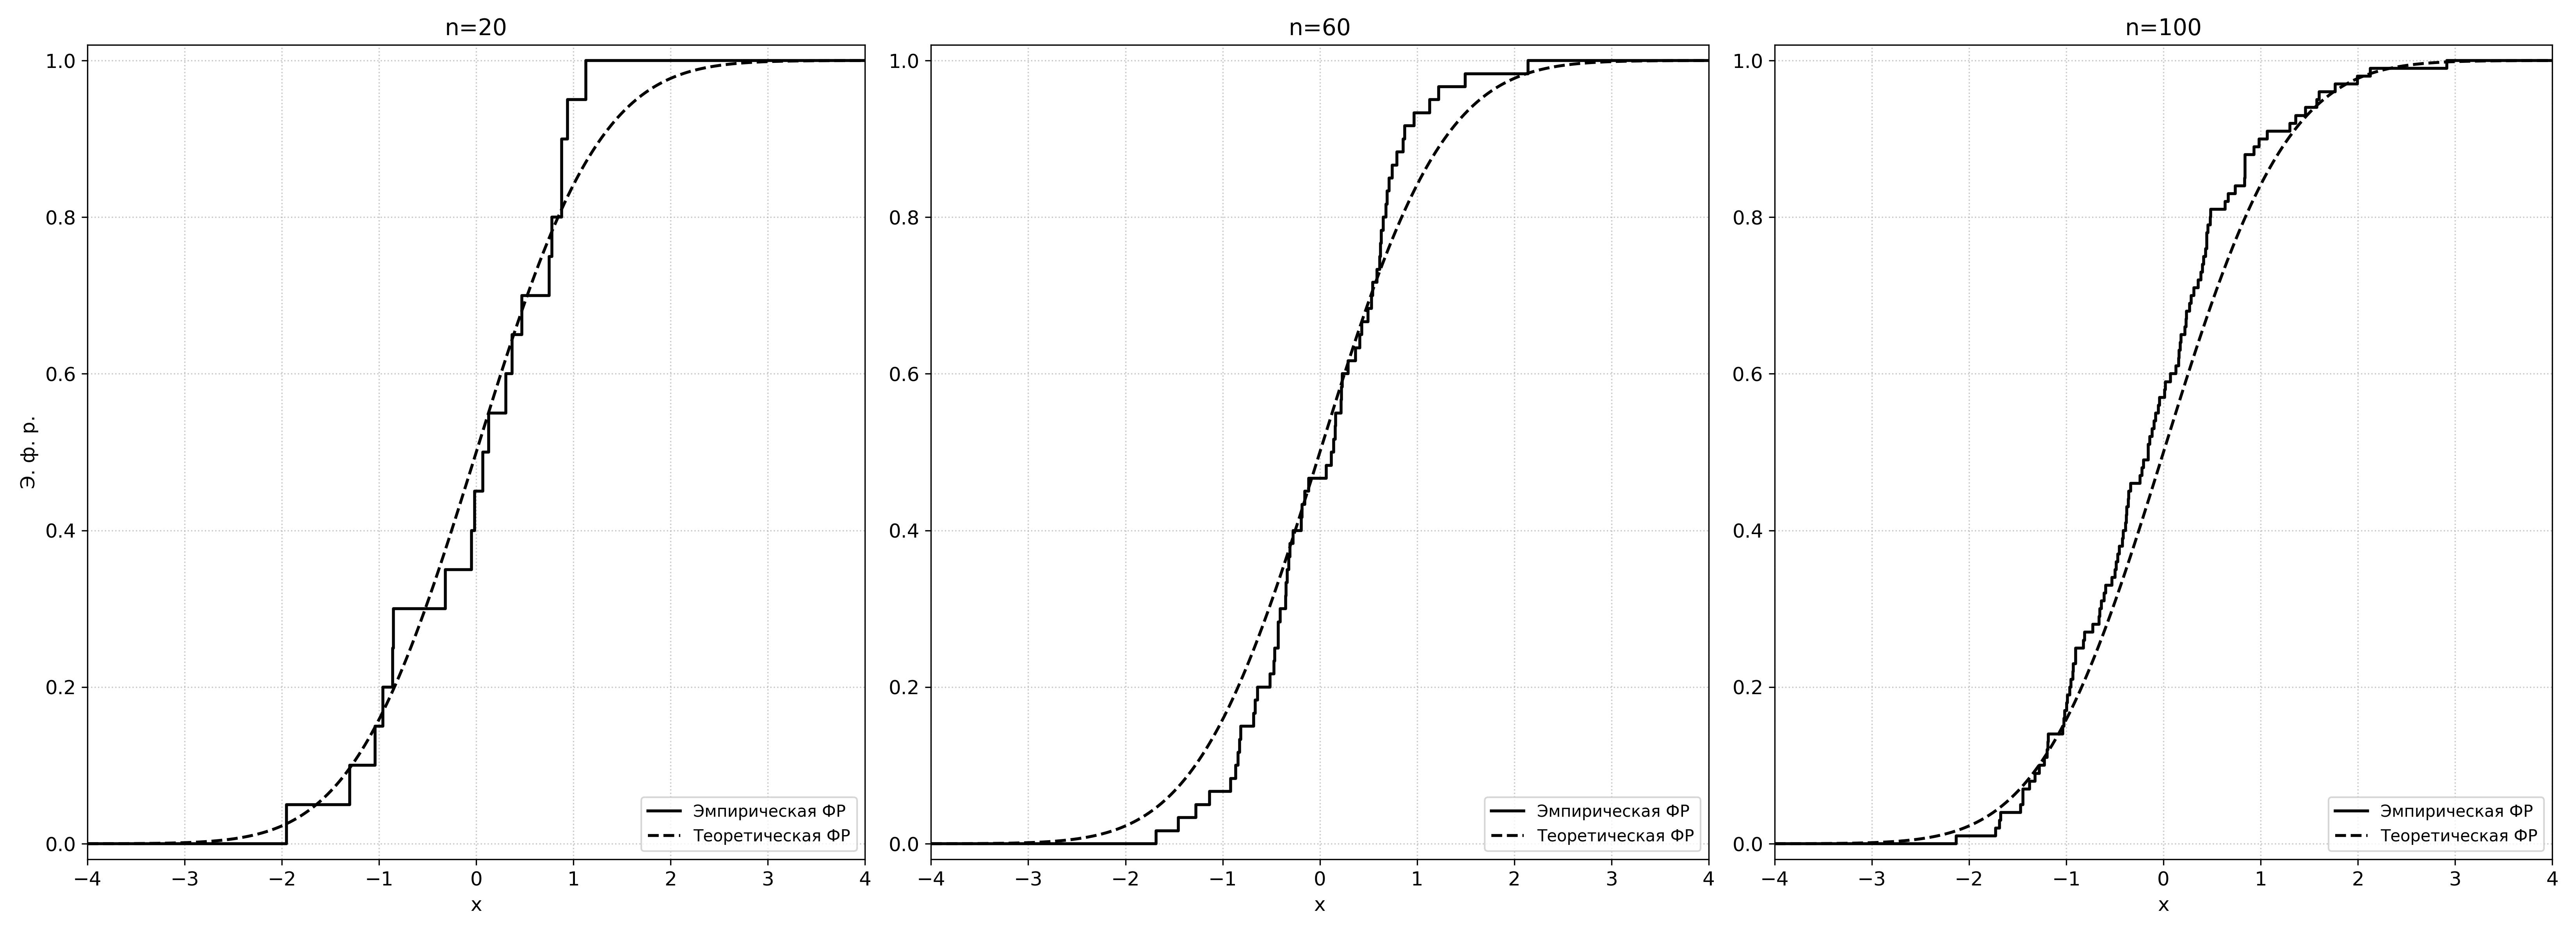
\includegraphics[width=\textwidth]{../figures/norm_ecdf.png}
        \caption{Эмпирическая и теоретическая функции распределения}
    \end{subfigure}
    \\
    \vspace{0.5em}
    \begin{subfigure}[t]{\textwidth}
        \centering
        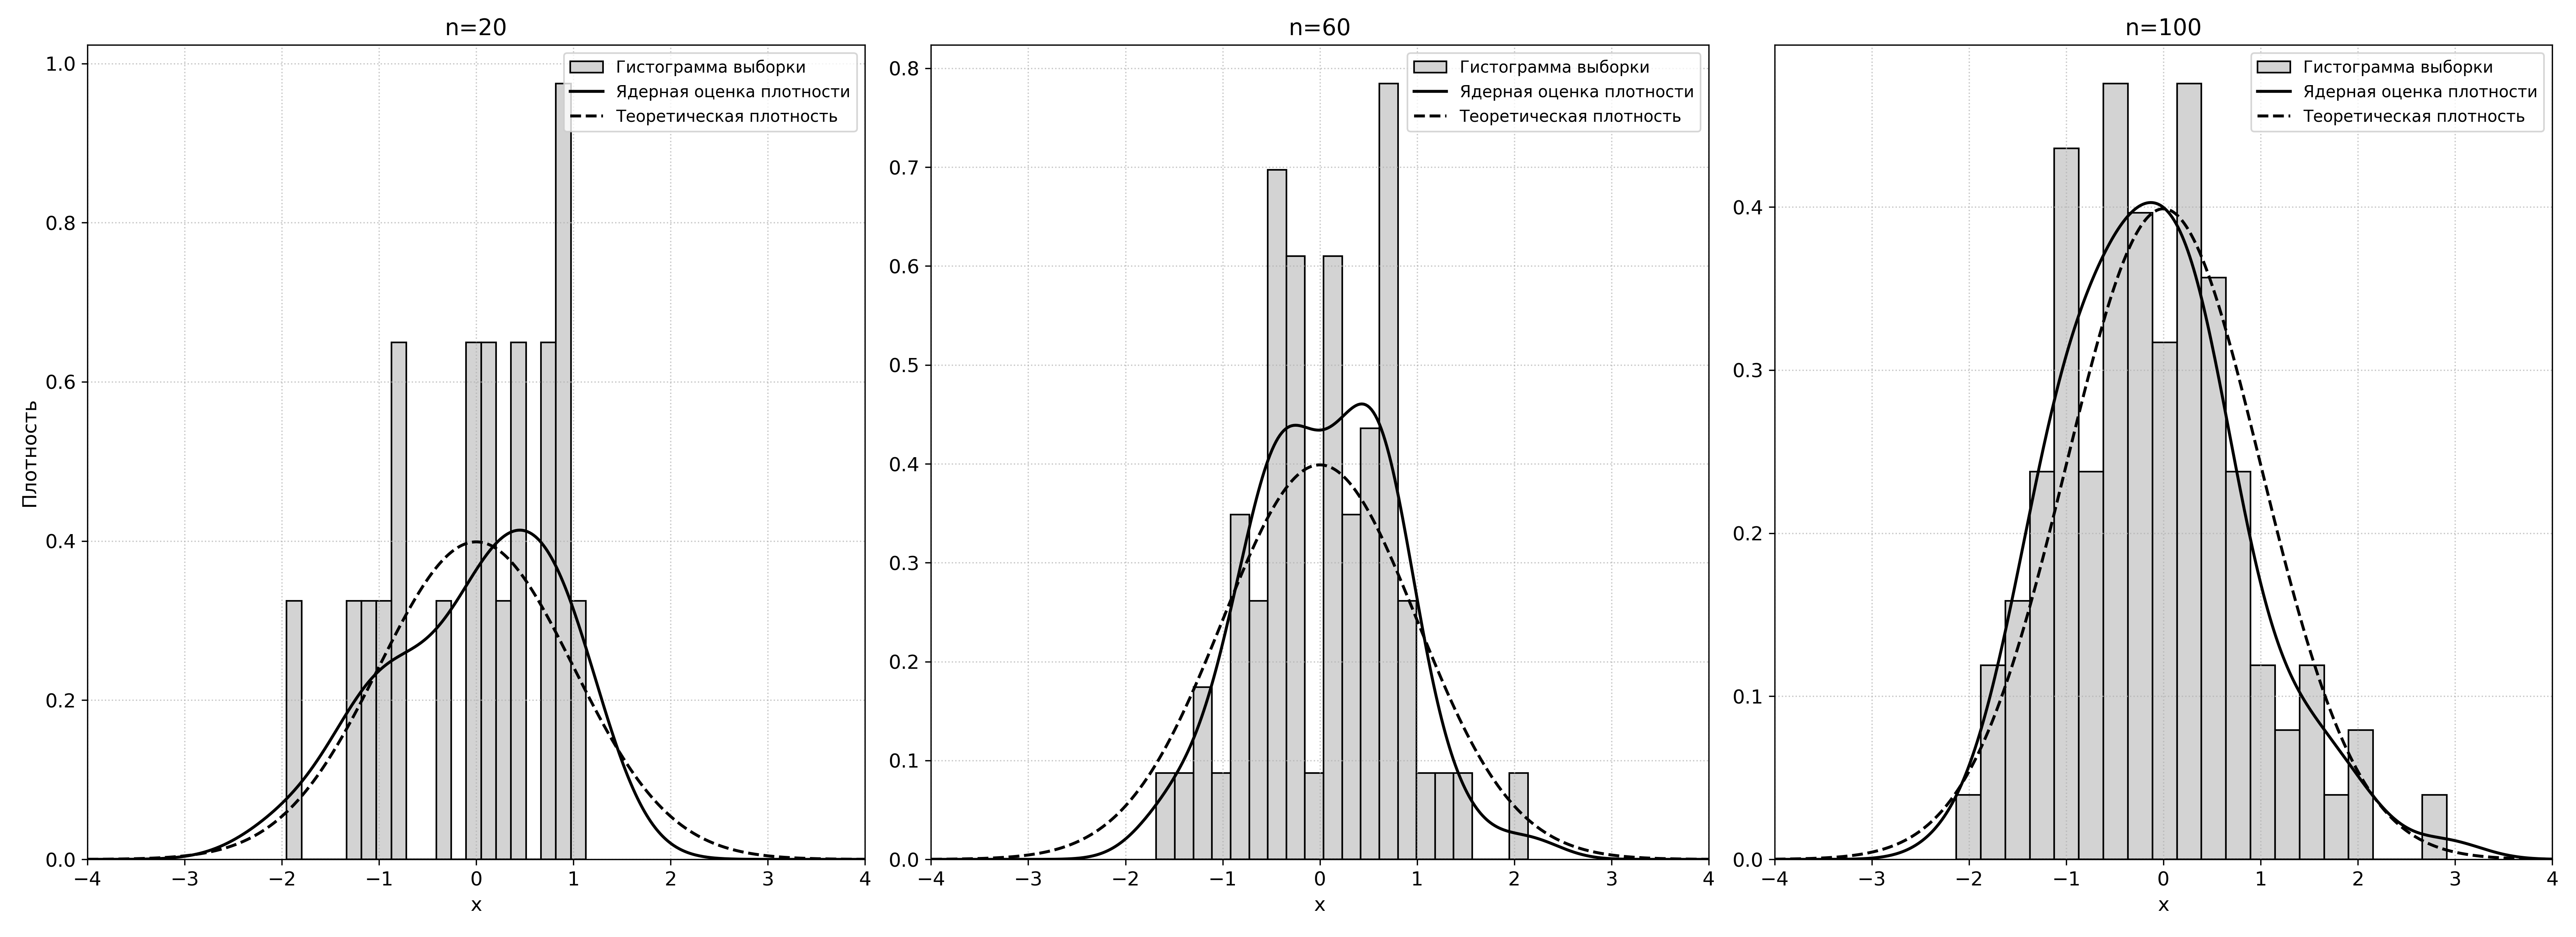
\includegraphics[width=\textwidth]{../figures/norm_density.png}
        \caption{Ядерная и теоретическая плотности}
    \end{subfigure}
    \caption{Графики для нормального распределения $N(0, 1)$}
    \label{fig:norm_pair}
\end{figure}

\begin{figure}[!htbp]
    \centering
    \begin{subfigure}[t]{\textwidth}
        \centering
        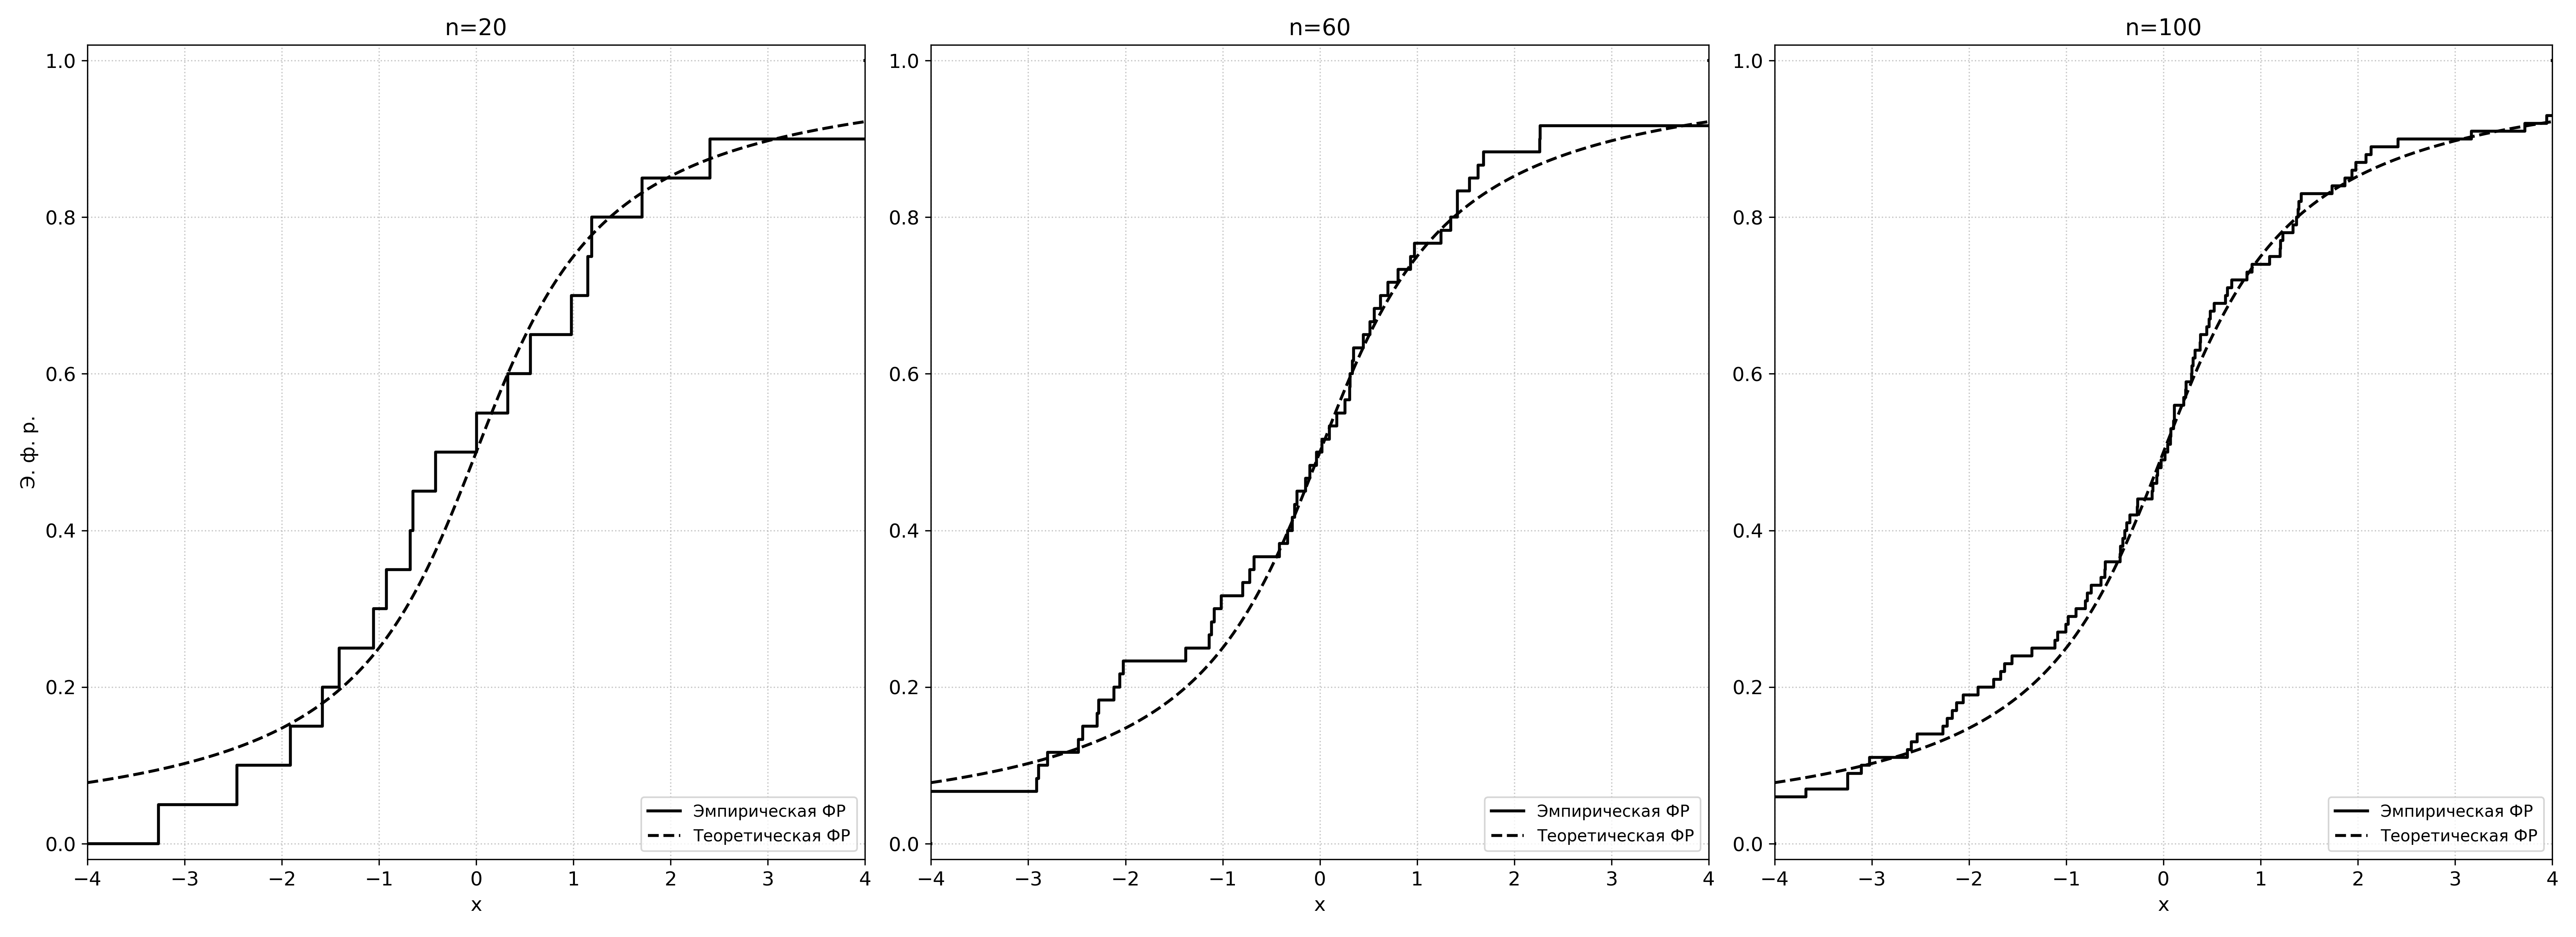
\includegraphics[width=\textwidth]{../figures/cauchy_ecdf.png}
        \caption{Эмпирическая и теоретическая функции распределения}
    \end{subfigure}
    \\
    \vspace{0.5em}
    \begin{subfigure}[t]{\textwidth}
        \centering
        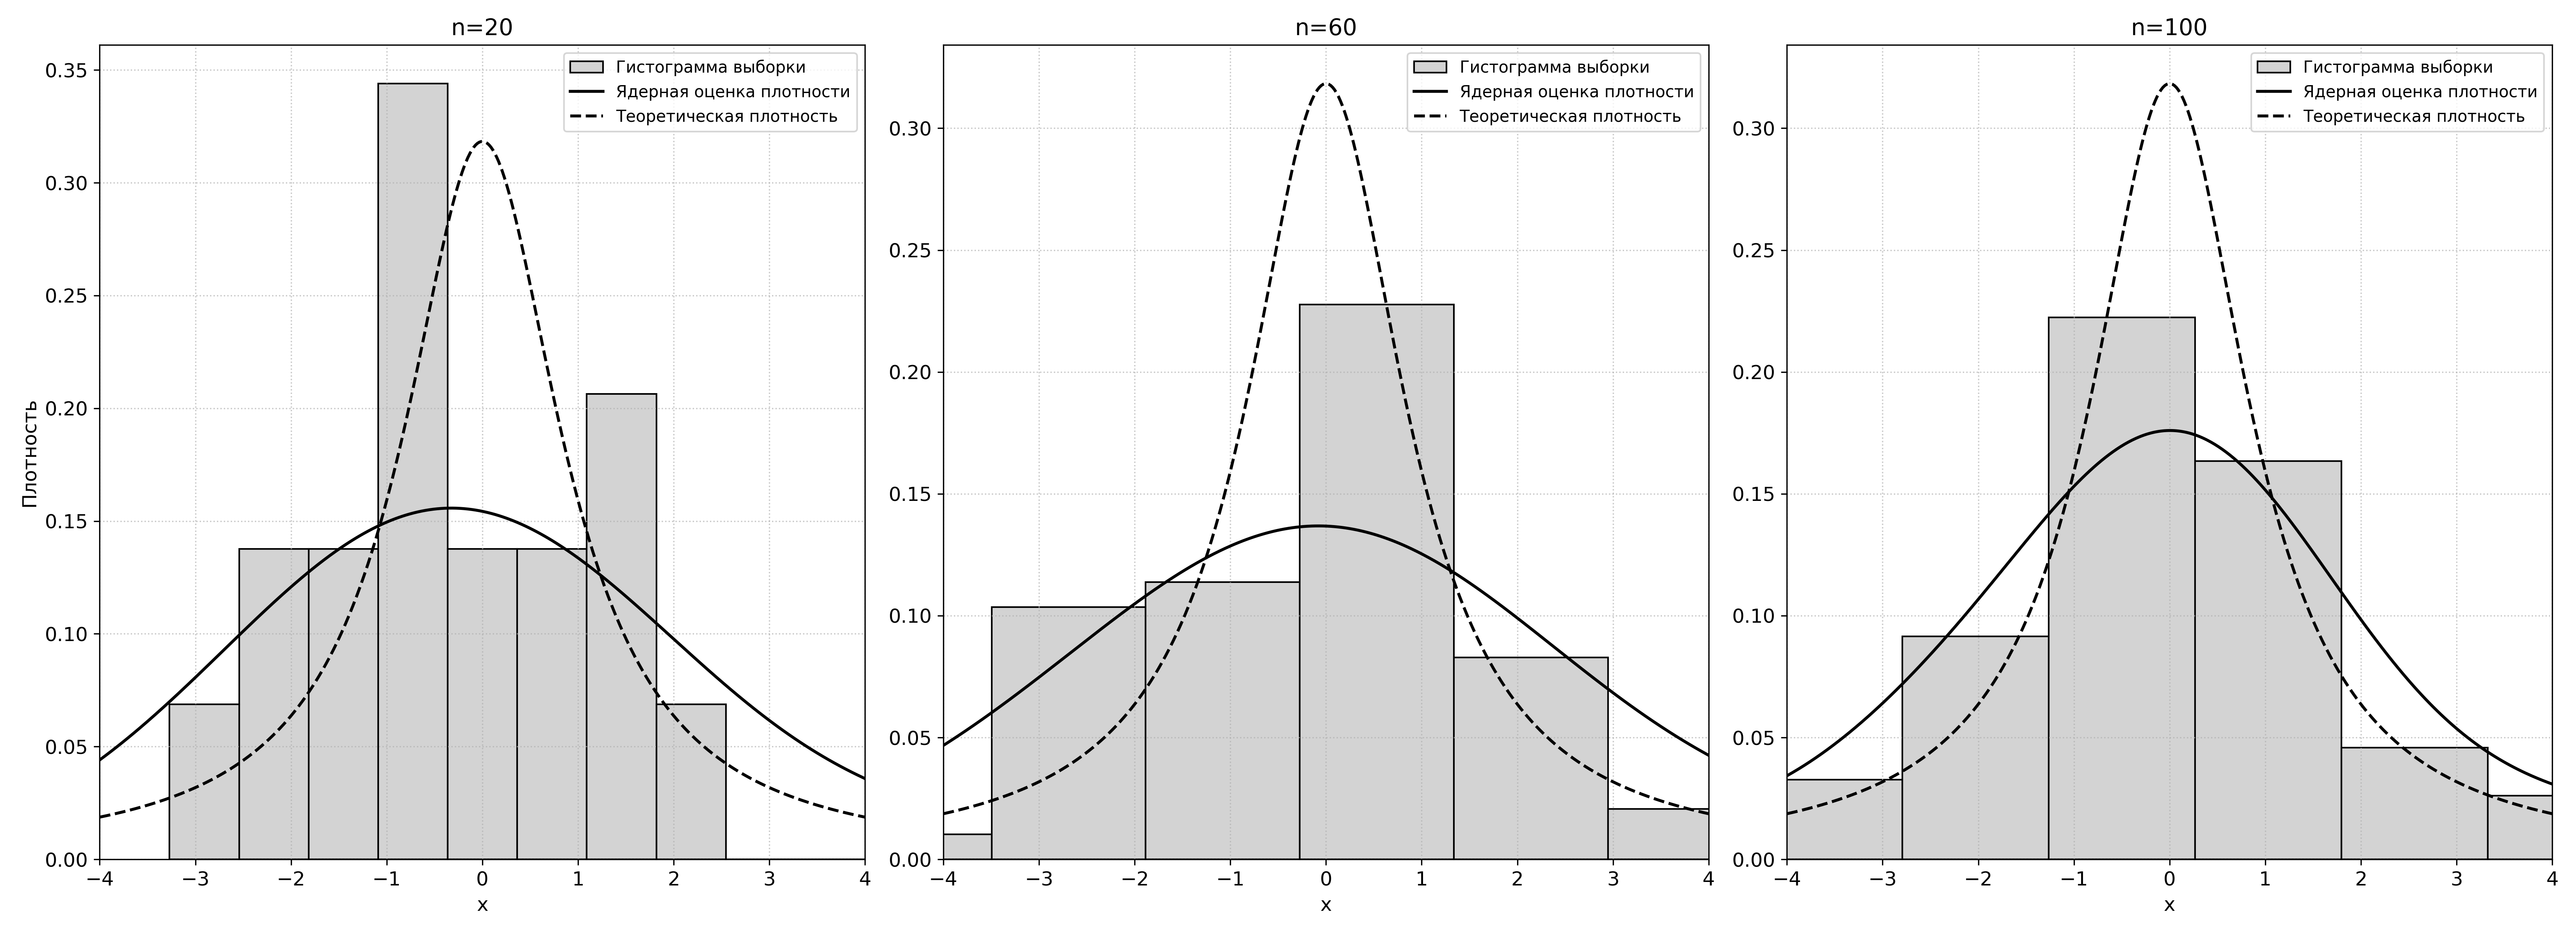
\includegraphics[width=\textwidth]{../figures/cauchy_density.png}
        \caption{Ядерная и теоретическая плотности}
    \end{subfigure}
    \caption{Графики для распределения Коши $C(0, 1)$}
    \label{fig:cauchy_pair}
\end{figure}

\begin{figure}[!htbp]
    \centering
    \begin{subfigure}[t]{\textwidth}
        \centering
        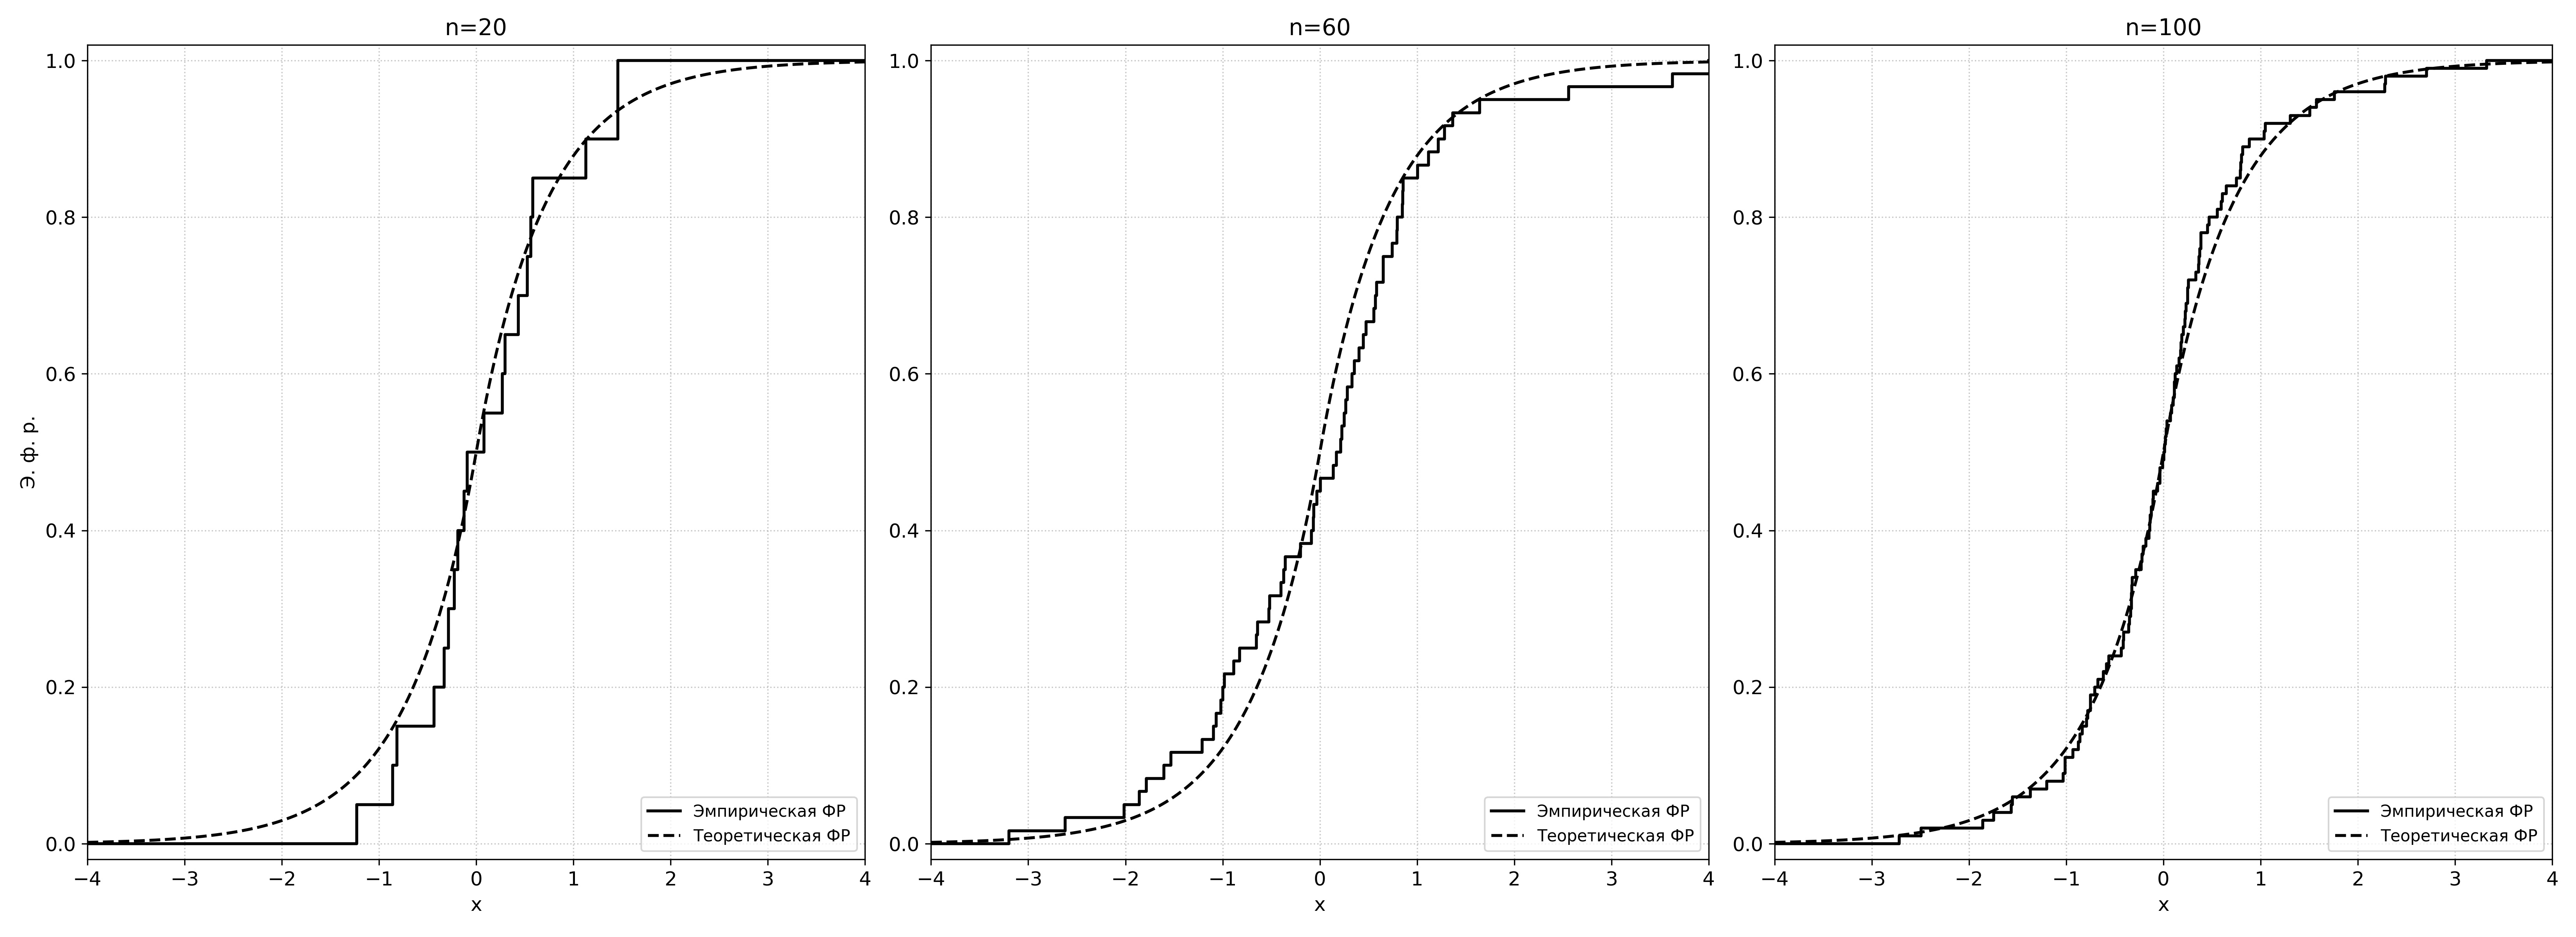
\includegraphics[width=\textwidth]{../figures/laplace_ecdf.png}
        \caption{Эмпирическая и теоретическая функции распределения}
    \end{subfigure}
    \\
    \vspace{0.5em}
    \begin{subfigure}[t]{\textwidth}
        \centering
        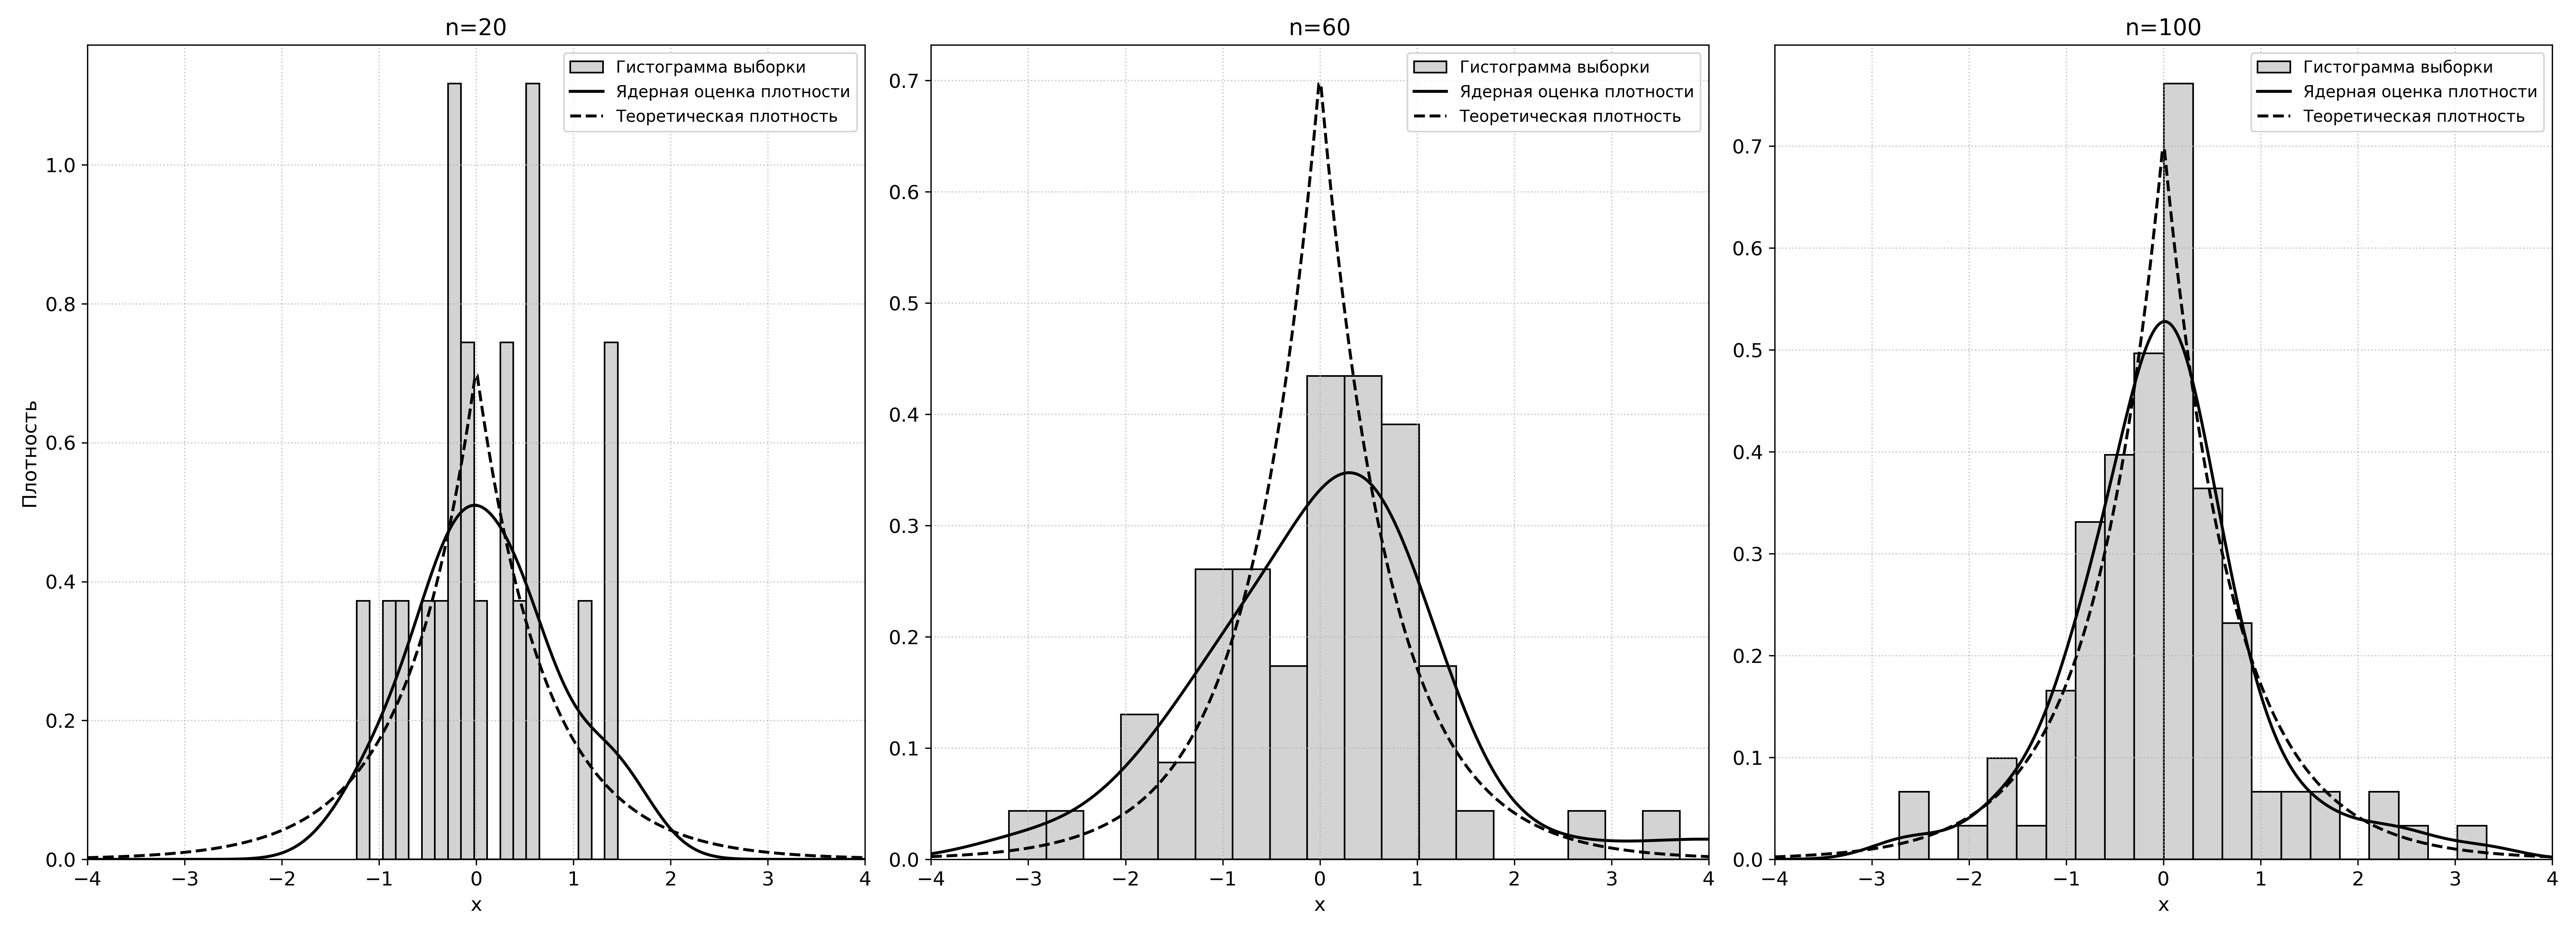
\includegraphics[width=\textwidth]{../figures/laplace_density.png}
        \caption{Ядерная и теоретическая плотности}
    \end{subfigure}
    \caption{Графики для распределения Лапласа $L(0, 1/\sqrt{2})$}
    \label{fig:laplace_pair}
\end{figure}

\begin{figure}[!htbp]
    \centering
    \begin{subfigure}[t]{\textwidth}
        \centering
        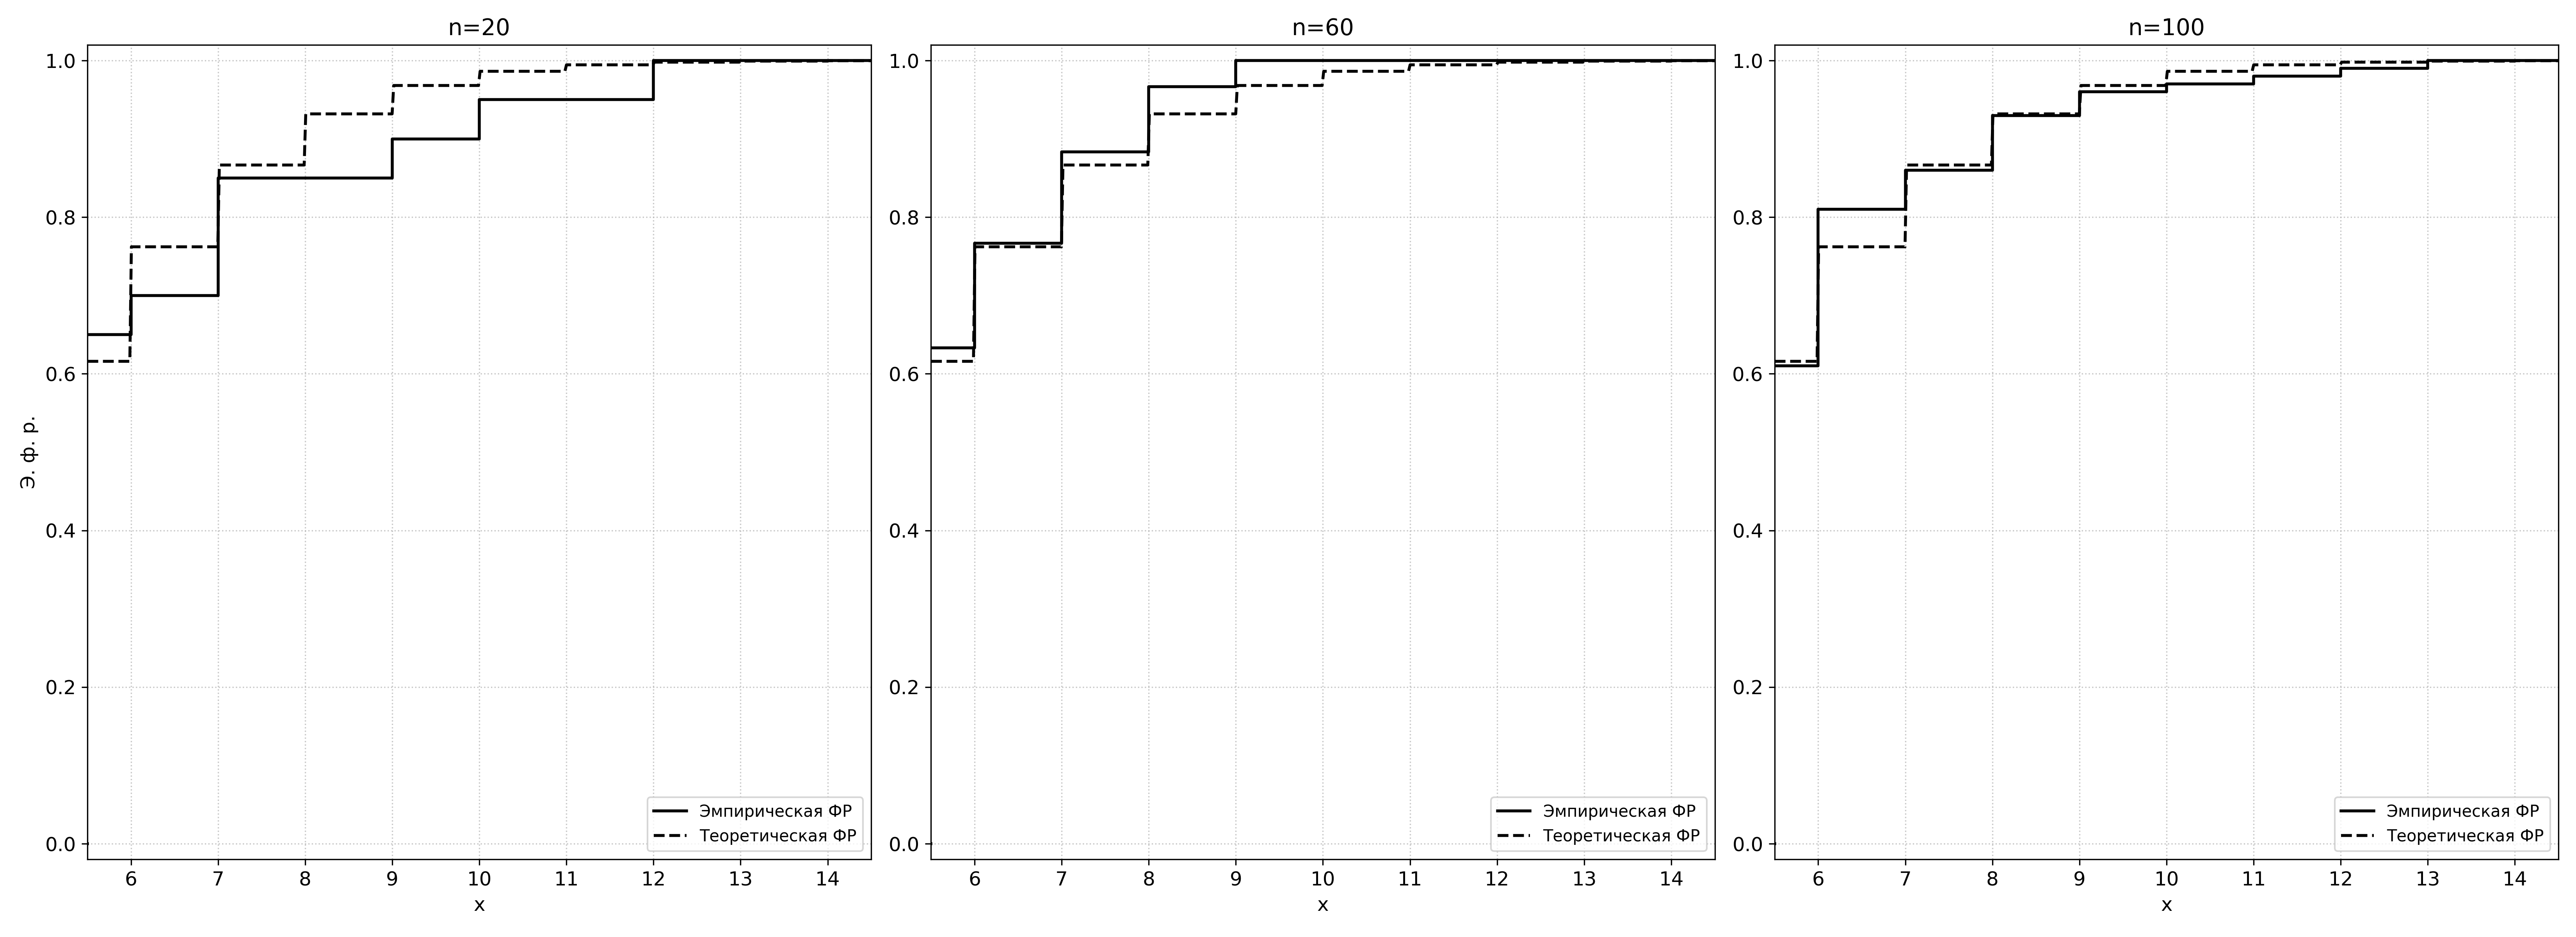
\includegraphics[width=\textwidth]{../figures/poisson_ecdf.png}
        \caption{Эмпирическая и теоретическая функции распределения}
    \end{subfigure}
    \\
    \vspace{0.5em}
    \begin{subfigure}[t]{\textwidth}
        \centering
        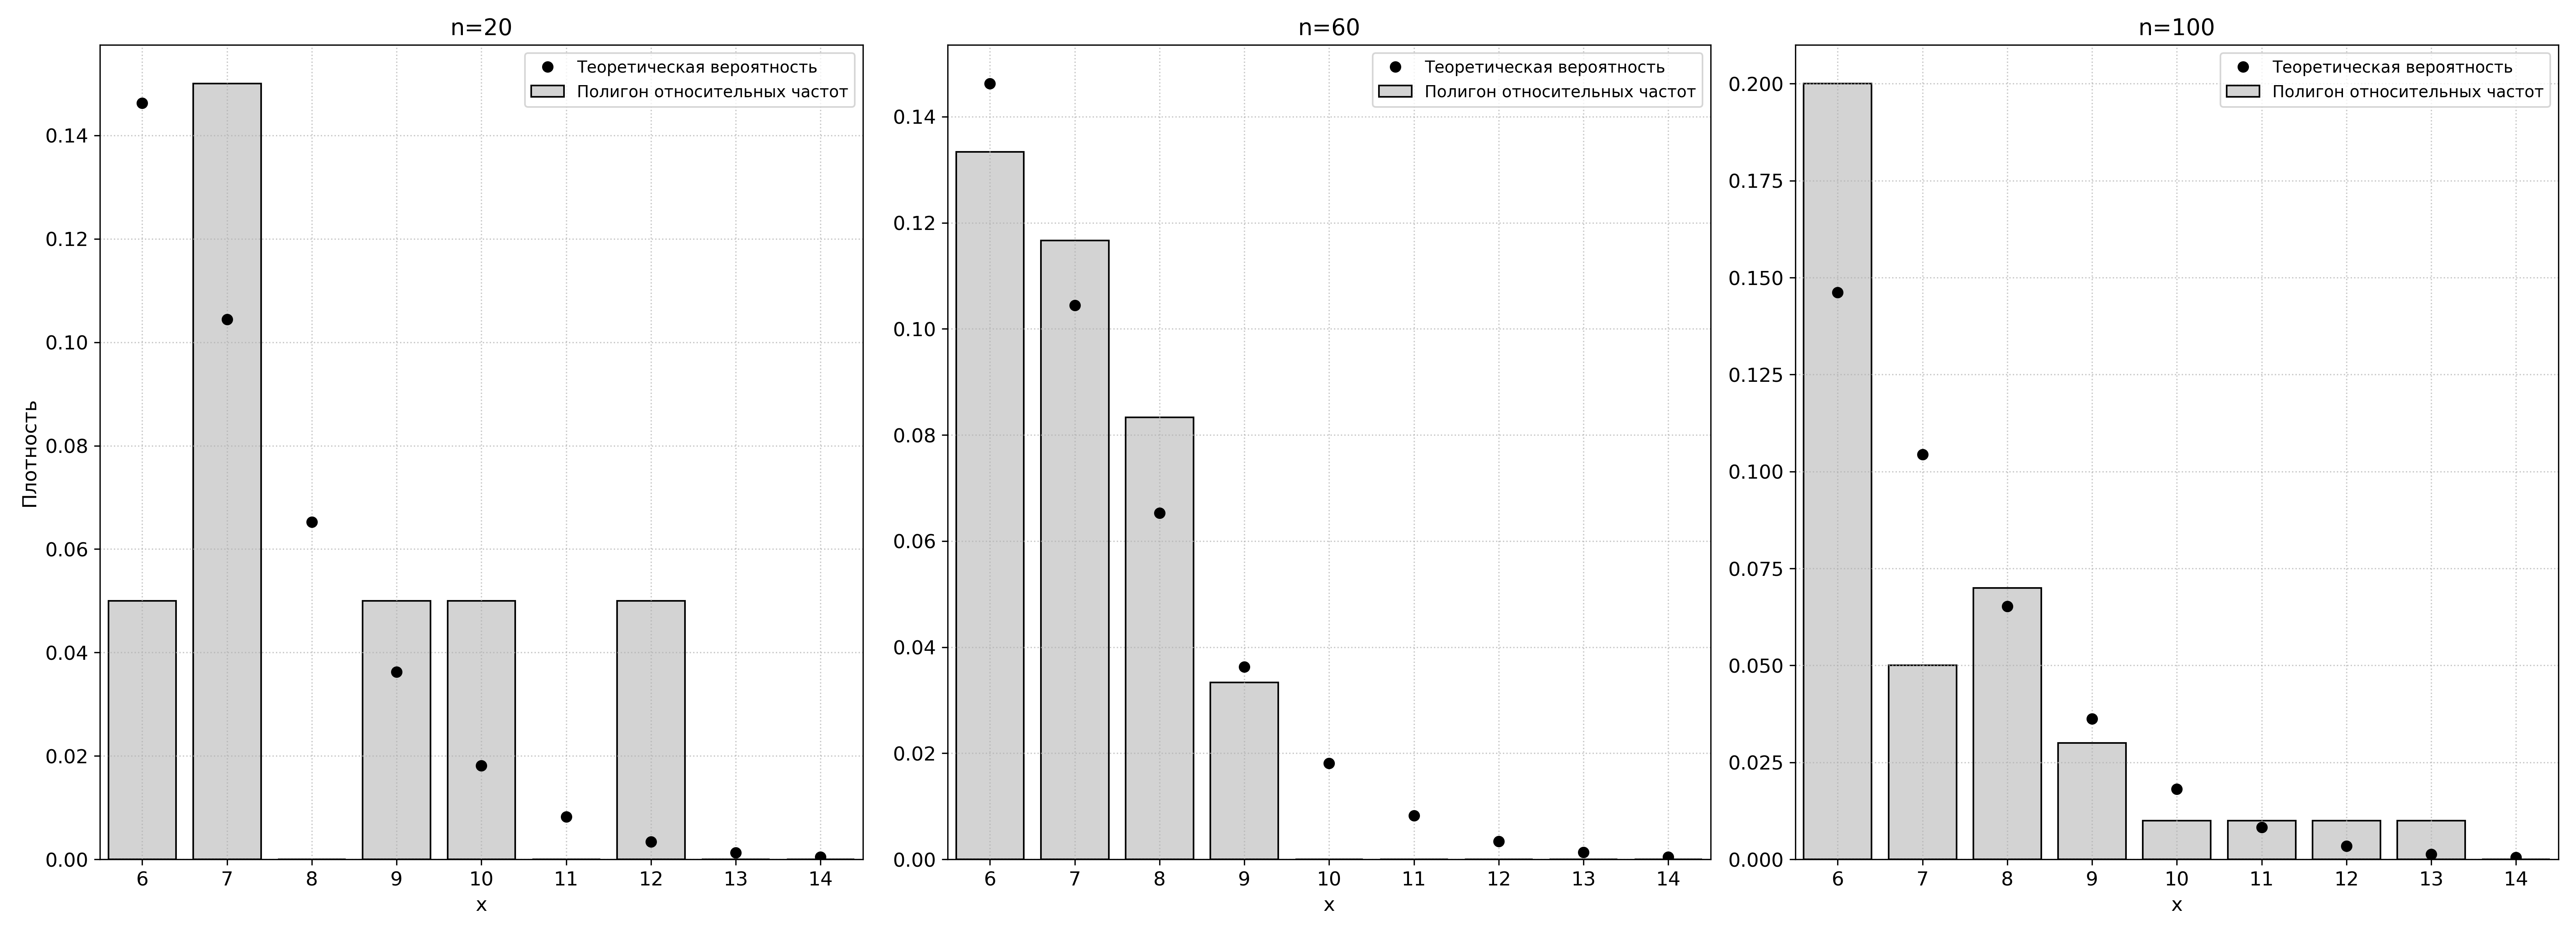
\includegraphics[width=\textwidth]{../figures/poisson_density.png}
        \caption{Полигон относительных частот и теоретическая вероятность}
    \end{subfigure}
    \caption{Графики для распределения Пуассона $P(5)$}
    \label{fig:poisson_pair}
\end{figure}

\begin{figure}[!htbp]
    \centering
    \begin{subfigure}[t]{\textwidth}
        \centering
        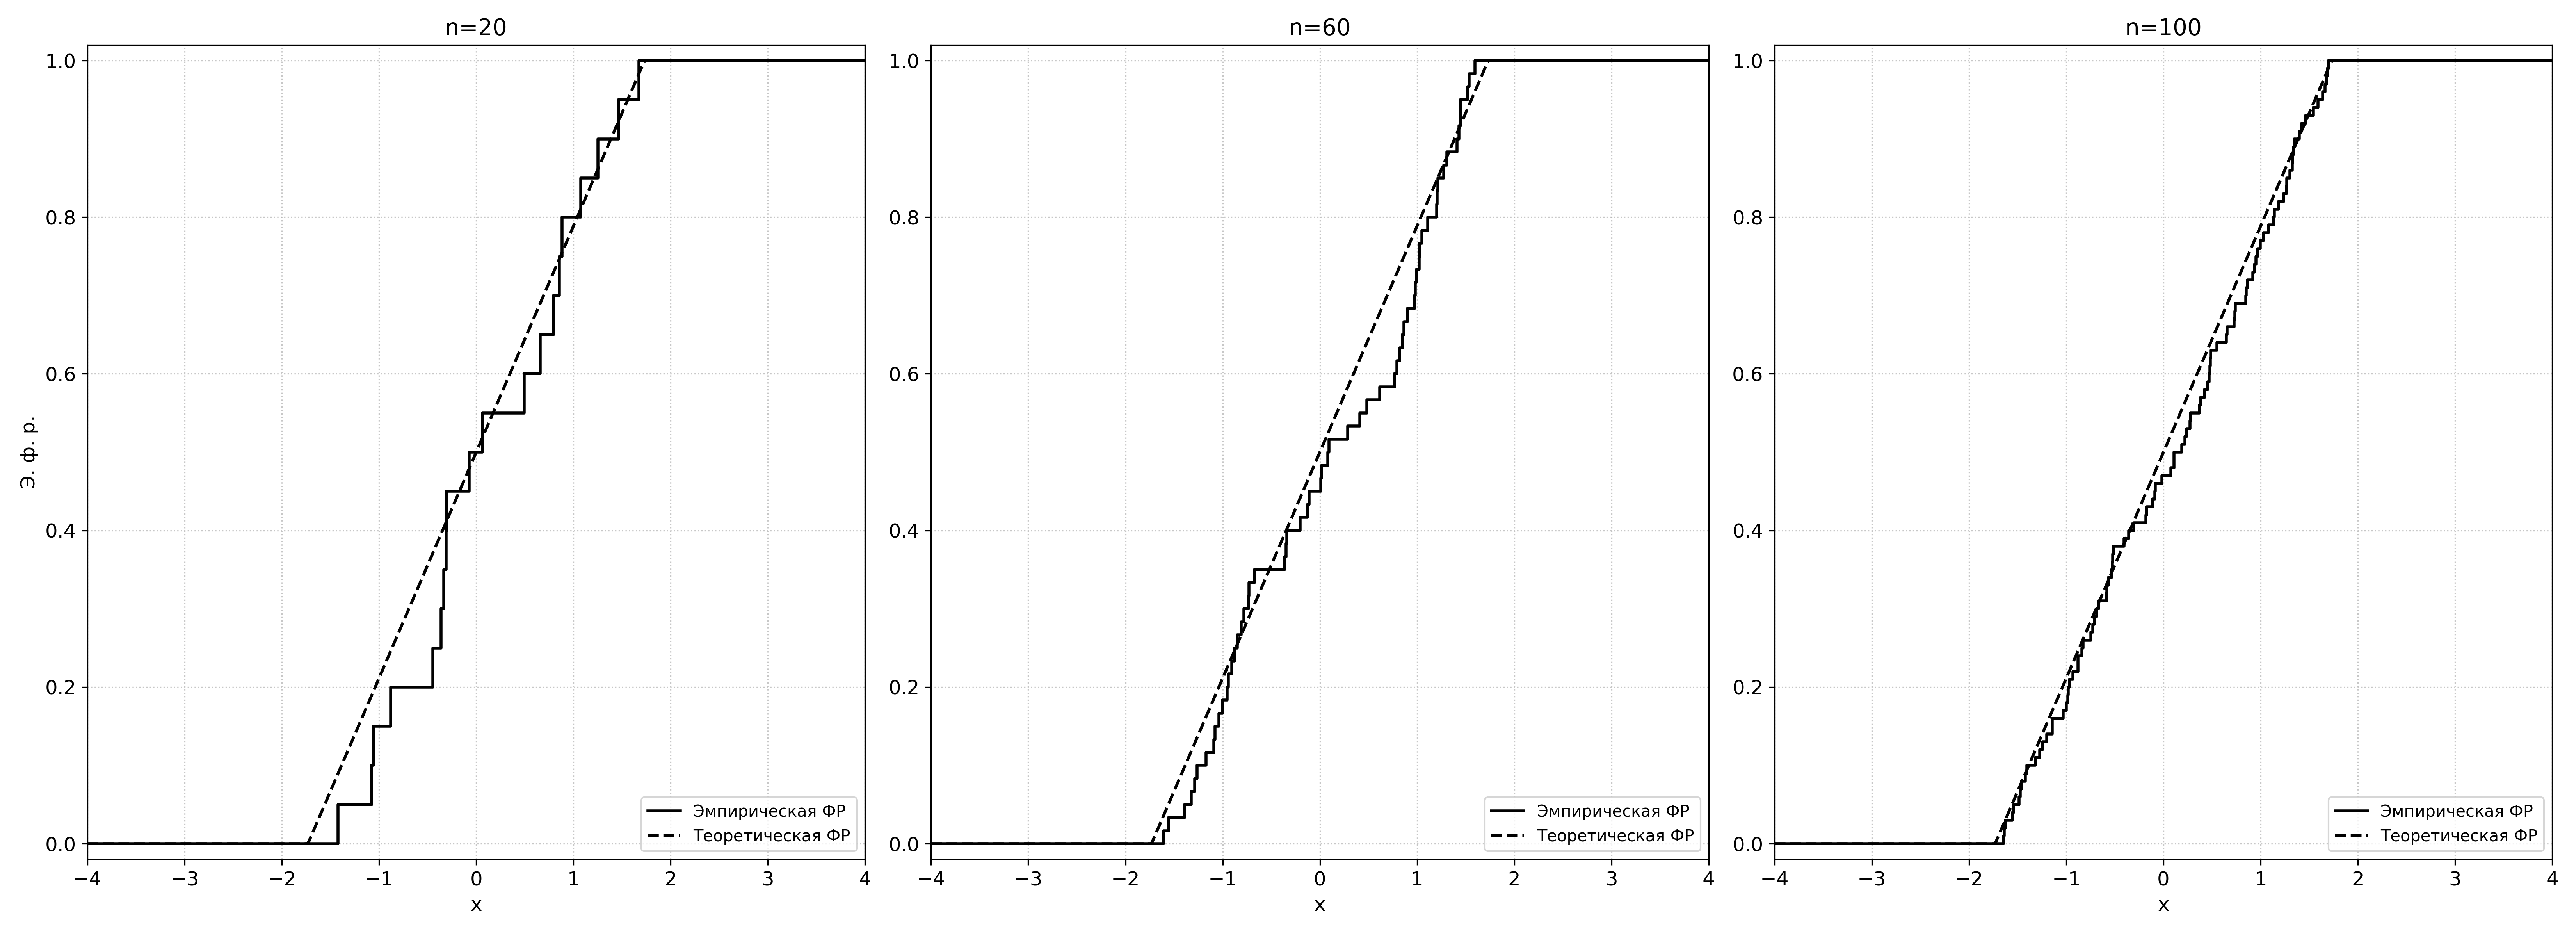
\includegraphics[width=\textwidth]{../figures/uniform_ecdf.png}
        \caption{Эмпирическая и теоретическая функции распределения}
    \end{subfigure}
    \\
    \vspace{0.5em}
    \begin{subfigure}[t]{\textwidth}
        \centering
        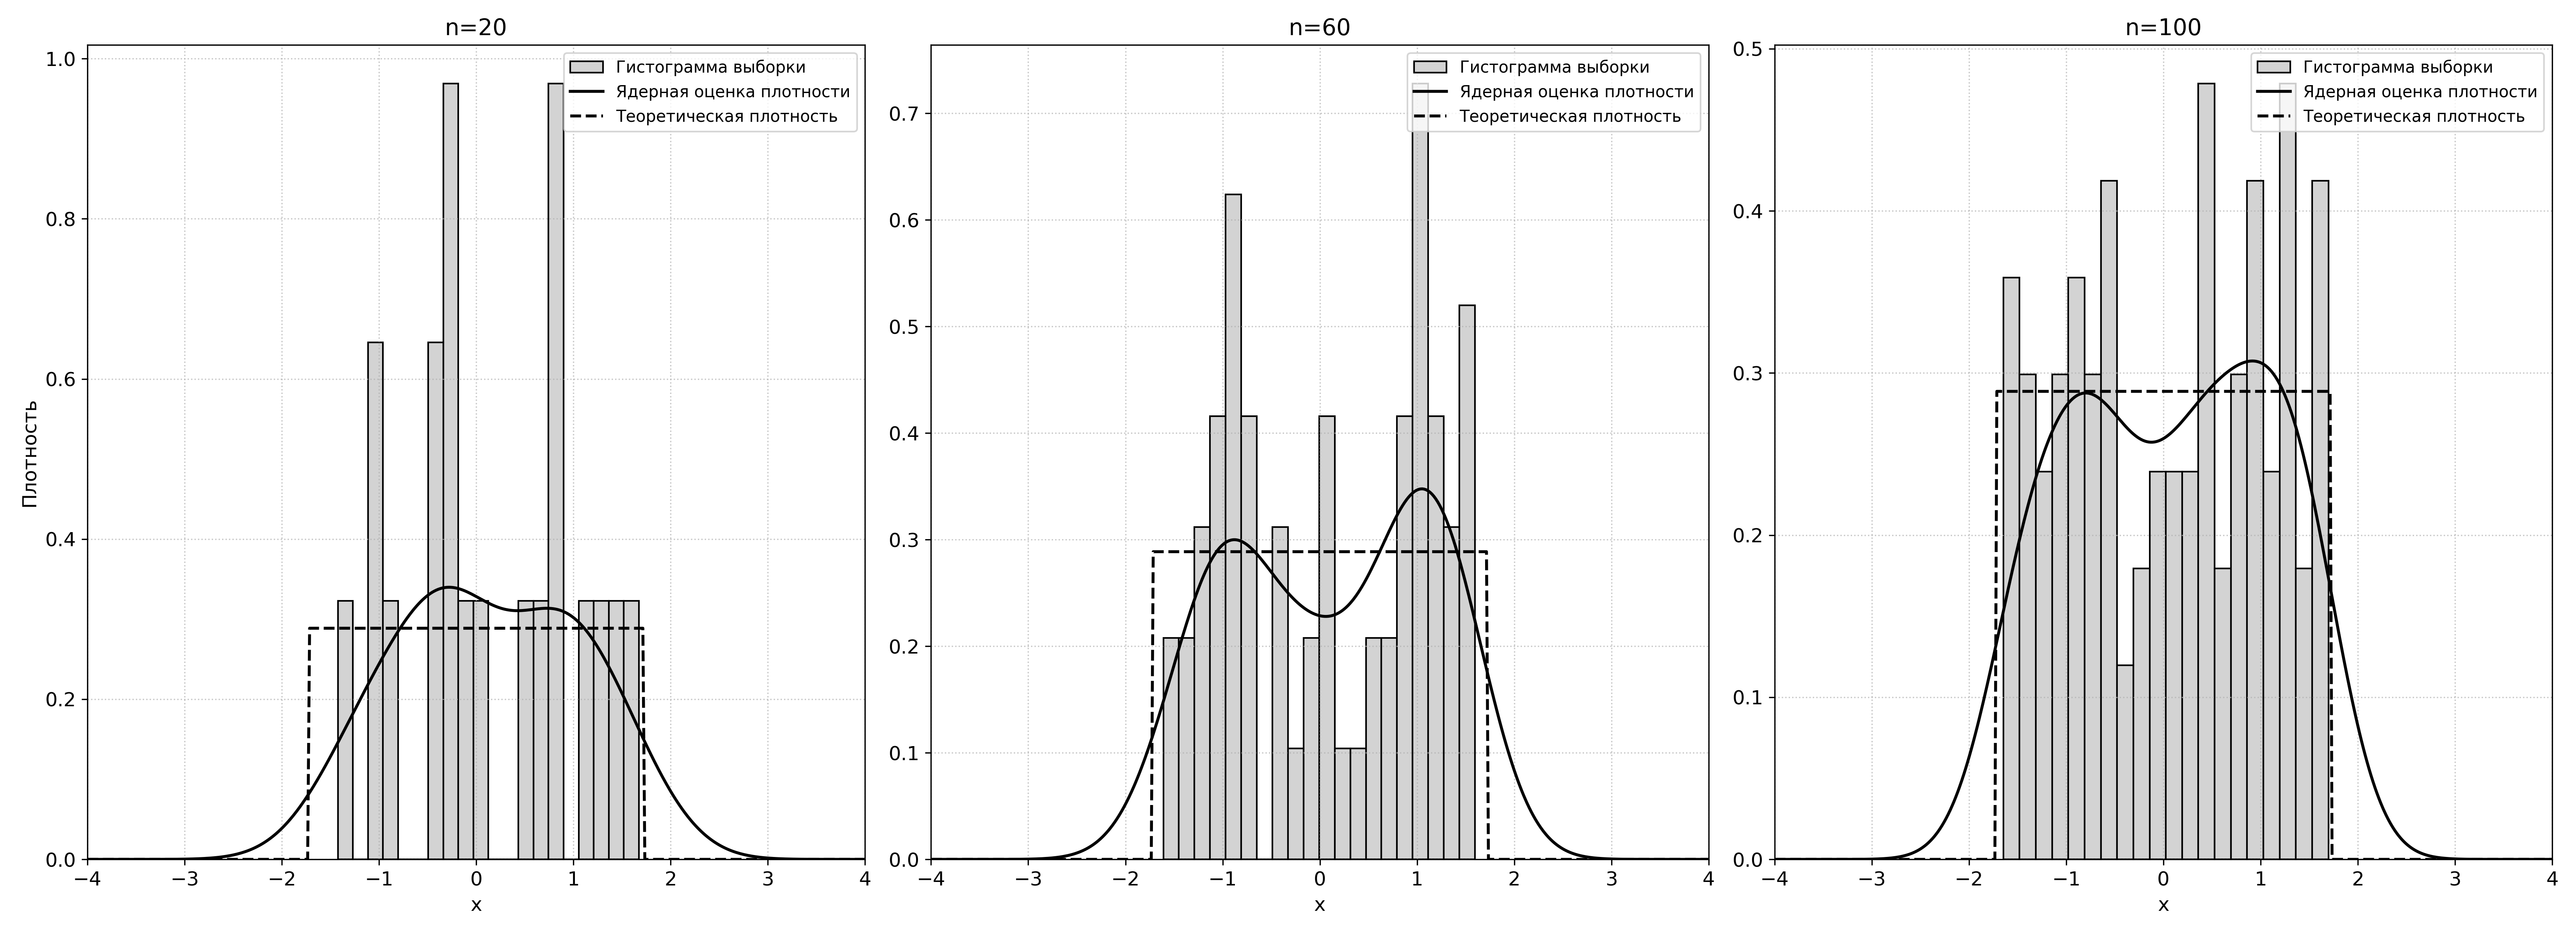
\includegraphics[width=\textwidth]{../figures/uniform_density.png}
        \caption{Ядерная и теоретическая плотности}
    \end{subfigure}
    \caption{Графики для равномерного распределения $U(-\sqrt{3}, \sqrt{3})$}
    \label{fig:uniform_pair}
\end{figure}

\FloatBarrier


\section{Обсуждение}

Анализ вычисленных метрик отклонения подтверждает теоретические положения о сходимости непараметрических оценок к генеральным функциям.

Максимальная абсолютная ошибка эмпирической функции распределения $D_n$ в большинстве случаев закономерно убывает с ростом $n$, что эмпирически доказывает теорему Гливенко-Кантелли о равномерной сходимости. Наиболее четко эта динамика отслеживается на распределениях без острых пиков и тяжелых хвостов в центральной части: для равномерного закона ошибка строго снижается с $0.1698$ при $n=20$ до $0.0513$ при $n=100$, для распределения Коши падает с $0.1338$ до $0.0580$. Зафиксированные локальные статистические колебания $D_n$ при переходе от $n=60$ к $n=100$ для нормального закона (рост с $0.1089$ до $0.1216$) и закона Пуассона ($0.0348 \to 0.0478$) обусловлены исключительно случайным характером генерации конкретных реализаций, однако абсолютные значения остаются в допустимых пределах статистической погрешности.

Точность ядерной оценки плотности ($MSE$) заметно зависит от формы хвостов распределения, поскольку именно она влияет на выбор ширины полосы $h$ по правилу Сильвермана. Для стандартного нормального закона алгоритм подбирает адекватный шаг сглаживания: среднеквадратичная ошибка минимальна и стабилизируется на уровне $0.0010$ при $n=100$. Для равномерного закона также получено достаточно точное приближение ($MSE = 0.0020$).

На распределении Коши качество аппроксимации заметно ниже. Тяжелые хвосты увеличивают выборочное стандартное отклонение $\hat{\sigma}$, из-за чего правило Сильвермана задает более широкую полосу $h$ и возникает пересглаживание графика плотности. В результате $MSE$ для закона Коши в 2--3 раза выше, чем для нормального закона ($0.0048$ при $n=60$, $0.0028$ при $n=100$). Для распределения Лапласа гауссовское ядро частично сглаживает острый пик плотности в нуле, однако при $n=100$ итоговая ошибка остается небольшой ($0.0008$). 

В случае дискретного закона Пуассона полигон относительных частот хорошо согласуется с теоретической функцией вероятностей: расчетная ошибка $MSE$ мала и составляет $0.0001$ при $n=60$ и $0.0007$ при $n=100$. 
Сравнение ядерных оценок с гистограммами выявляет системные аналитические различия методов. Гистограмма представляет собой кусочно-постоянную аппроксимацию, чувствительную к шагу разбиения. KDE формирует строго непрерывную гладкую кривую. 

Для нормального закона и распределения Лапласа при $n=100$ ядерное сглаживание дает визуально более точное совпадение с теоретической плотностью, полностью устраняя ступенчатые артефакты гистограмм. Однако на границах финитных законов метод дает сбой. Для равномерного распределения $U(-\sqrt{3}, \sqrt{3})$ суперпозиция гауссовских ядер генерирует фиктивные вероятностные «хвосты» за пределами интервала $[-\sqrt{3}, \sqrt{3}]$. Гистограмма в данном случае точнее отражает отсутствие вероятностной массы за границами отрезка. 

При анализе распределения Коши $C(0, 1)$ гистограмма уверенно локализует центральный пик даже при наличии выбросов. Ядерная оценка с этим не справляется: аномальный рост выборочного стандартного отклонения $\hat{\sigma}$ из-за тяжелых хвостов приводит к завышению параметра $h$ и критическому пересглаживанию кривой KDE.


\section{Выводы}

Методами статистического моделирования исследована сходимость эмпирических функций распределения (ЭФР) и ядерных оценок плотности (KDE).

Экспериментально подтверждено, что ЭФР является универсальным инструментом непараметрического анализа одномерных данных. С увеличением объема выборки до $n=100$ статистика Колмогорова $D_n$ снижается, обеспечивая надежное приближение к истинной функции распределения независимо от ее аналитического вида.

Установлено, что точность ядерного сглаживания с применением гауссовского ядра и правила Сильвермана зависит от структуры хвостов распределения. Для законов с экспоненциальными и финитными хвостами (Нормальное, Равномерное, Лапласа) метод обеспечивает хорошее качество аппроксимации и малую среднеквадратичную ошибку ($MSE \le 0.0020$). Для распределения Коши наблюдается пересглаживание из-за увеличенной полосы пропускания $h$, что ухудшает восстановление истинной плотности вероятности. Сравнительный анализ методов восстановления плотности показал, что ядерное сглаживание (KDE) превосходит классические гистограммы при аппроксимации непрерывных распределений с экспоненциально убывающими хвостами. При анализе финитных законов (Равномерное) и распределений без конечных моментов (Коши) KDE уступает гистограммам из-за краевых эффектов и неробастности алгоритма вычисления ширины полосы $h$, что приводит к искажению истинной формы генеральной плотности.
\refstepcounter{section}
\addcontentsline{toc}{section}{\thesection\ Список литературы}
\renewcommand{\refname}{\thesection\ Список литературы}

\begin{thebibliography}{9}

    \bibitem{babakhina}
    Бабахина С. А., Баженов А. Н. Практикум по математической статистике: учеб. пособие. — СПб. : Санкт-Петербургский политехнический университет Петра Великого, 2026. 

    \bibitem{maksimov}
    Максимов Ю. Д. Математика. Теория и практика по математической статистике. Конспект-справочник по теории вероятностей : учеб. пособие. — СПб. : Изд-во Политехн. ун-та, 2009. — 395 с. 

\end{thebibliography}

\section{Приложение}

Исходный код программ доступен в репозитории на GitHub: \\
\url{https://github.com/Reichenau/math-stats-labs}
 
\end{document}
